\documentclass[10pt,letterpaper,onecolumn,journal]{IEEEtran}
\usepackage[margin=0.75in]{geometry}
\usepackage{listings}
\usepackage{color}
\usepackage{longtable}
\usepackage{graphicx}
\usepackage{float}
\usepackage{courier}
\usepackage[hidelinks]{hyperref}
\usepackage{tikz}
\usetikzlibrary{shapes.geometric, arrows}

\floatstyle{boxed}
\restylefloat{figure}
\setlength{\parindent}{0cm}

\begin{document}
\pagenumbering{arabic}

\title{Winter Progress Report\\ARLISS Micro-Satellite Project}
\author{Paul Minner\\Capstone Group 27}
\maketitle

\section{Introduction}
Autonomous navigation has become a hot topic lately since many car companies have implemented some level of autonomous driving in their new vehicles. Our project combines the idea of autonomous navigation with rocketry to create an autonomously navigated rover. Our task is to create a rover capable of being launched 12,000 feet above ground level, parachute to the ground, and autonomously navigate to a set of GPS coordinates while avoiding obstacles in it's path. We will be competing with other rovers in a competition called ARLISS. To accomplish this feat, we have grouped with a team of mechanical and electrical engineers to complete the hardware requirements, while we, the computer science team, work on the software. 

\section{Individual Pieces}
Originally, I was responsible for parachute deployment, getting unstuck from obstacles, and touching the finish pole. The parachute deployment module ensures we deploy the parachute a safe distance above the ground, but not so far above the ground that we drift far from the finish due to wind. The getting unstuck from obstacles module determines if the rover has hit an obstacle and is not moving, then attempts to move the rover in another direction so it can continue it's journey. Finally, the touching the finish pole module attempts to drive the rover into the finish pole at the GPS coordinates. This module is needed because GPS is only accurate to roughly 8 meters, so within those 8 meters, we have to locate the position of the pole within an image taken by the on-board camera and drive into it. Another member of the team is responsible for finding the pole in the image. I finished the majority of the functionality for these modules at the beginning of this term, so this half of the term I have focused on integrating our software onto the raspberry pi zero, as well as merging our team's separate modules into one coherent program. 

\section{Progress and Problems}
Previously this term, my greatest problem was the fact that I couldn't test any of my modules on the hardware we were going to use. This half of the term, we finally got access to the raspberry pi zero and camera, so I could run my modules on some of the hardware. Unfortunately, we still haven't got access to the completed rover, so I've been unable to test my modules using actual GPS coordinates and motors, which would have been more useful than just the raspberry pi. For this reason, I haven't changed my initial modules much from what they were since our last progress report, because I won't know how well they work until we can test the completed rover.\vspace{.3cm}
\par
This term, I focused more on integrating our software onto the raspberry pi and merging the entire team's separate modules into a single program runnable on the pi. Originally, Zach was planning to implement the framework, which would include merging everybody's modules, but he is also responsible for the image sensing, which has turned out to be more difficult than we expected, so I am working on merging the program now. To accomplish this, I implemented each person's modules as separate classes, and created a parent class so that information could be shared between modules, such as image data, or GPS coordinates. Merging the modules this way also allowed me to easily write better testing functions for returning GPS coordinates and motor control functions, so that all the modules could use the same functions. Previously, everybody tested their code using separate functions to simulate the functionality of the hardware that we don’t have. In addition, some modules work within other modules, such as the obstacle avoidance module working within the GPS navigation module. Implementing each module as a class and creating a class hierarchy allows us to easily accomplish this. My only issue so far regarding this part of the project is that some modules are still incomplete, so I am unable to make the program completely functional yet, although it is very close.\vspace{.3cm}
\par
The other aspect of the project I focused on this half of the term was integrating the software onto the raspberry pi. We received the pi soon after the first progress report was due this term, and I've been responsible for getting it up and running. To do that, first I had to boot the operating system. We purchased a Micro SD card with the operating system installed, so that wasn’t a problem. I also had to obtain hardware to run the pi, like a Mini-HDMI cable, Micro-USB adapter, and USB Hub. None of these components are needed on the rover itself, but in order to navigate the operating system to set up the software for the rover, a video connection, keyboard, and mouse are all required. Once the pi was booted, I was able to compile our software on the pi, as well as install OpenCV, an important library we use for object detection. Lastly, I created a script which runs as soon as the pi boots. This script executes our program, and shuts the pi down once the program is finished. This is very important because we have no way to start the program on the rover unless we plug in a monitor and keyboard, which is not possible at the competition. I had hoped to test the software on the finished rover by the end of this term, but unfortunately, the hardware components won't be finished until Thursday of finals week, so we have no time to test the completed rover this term. We should be able to get the completed rover up and running immediately next term, so we can start testing, which is very important.\vspace{.3cm}

\floatstyle{plain}
\restylefloat{figure}
\begin{figure}[h]
  \centering
  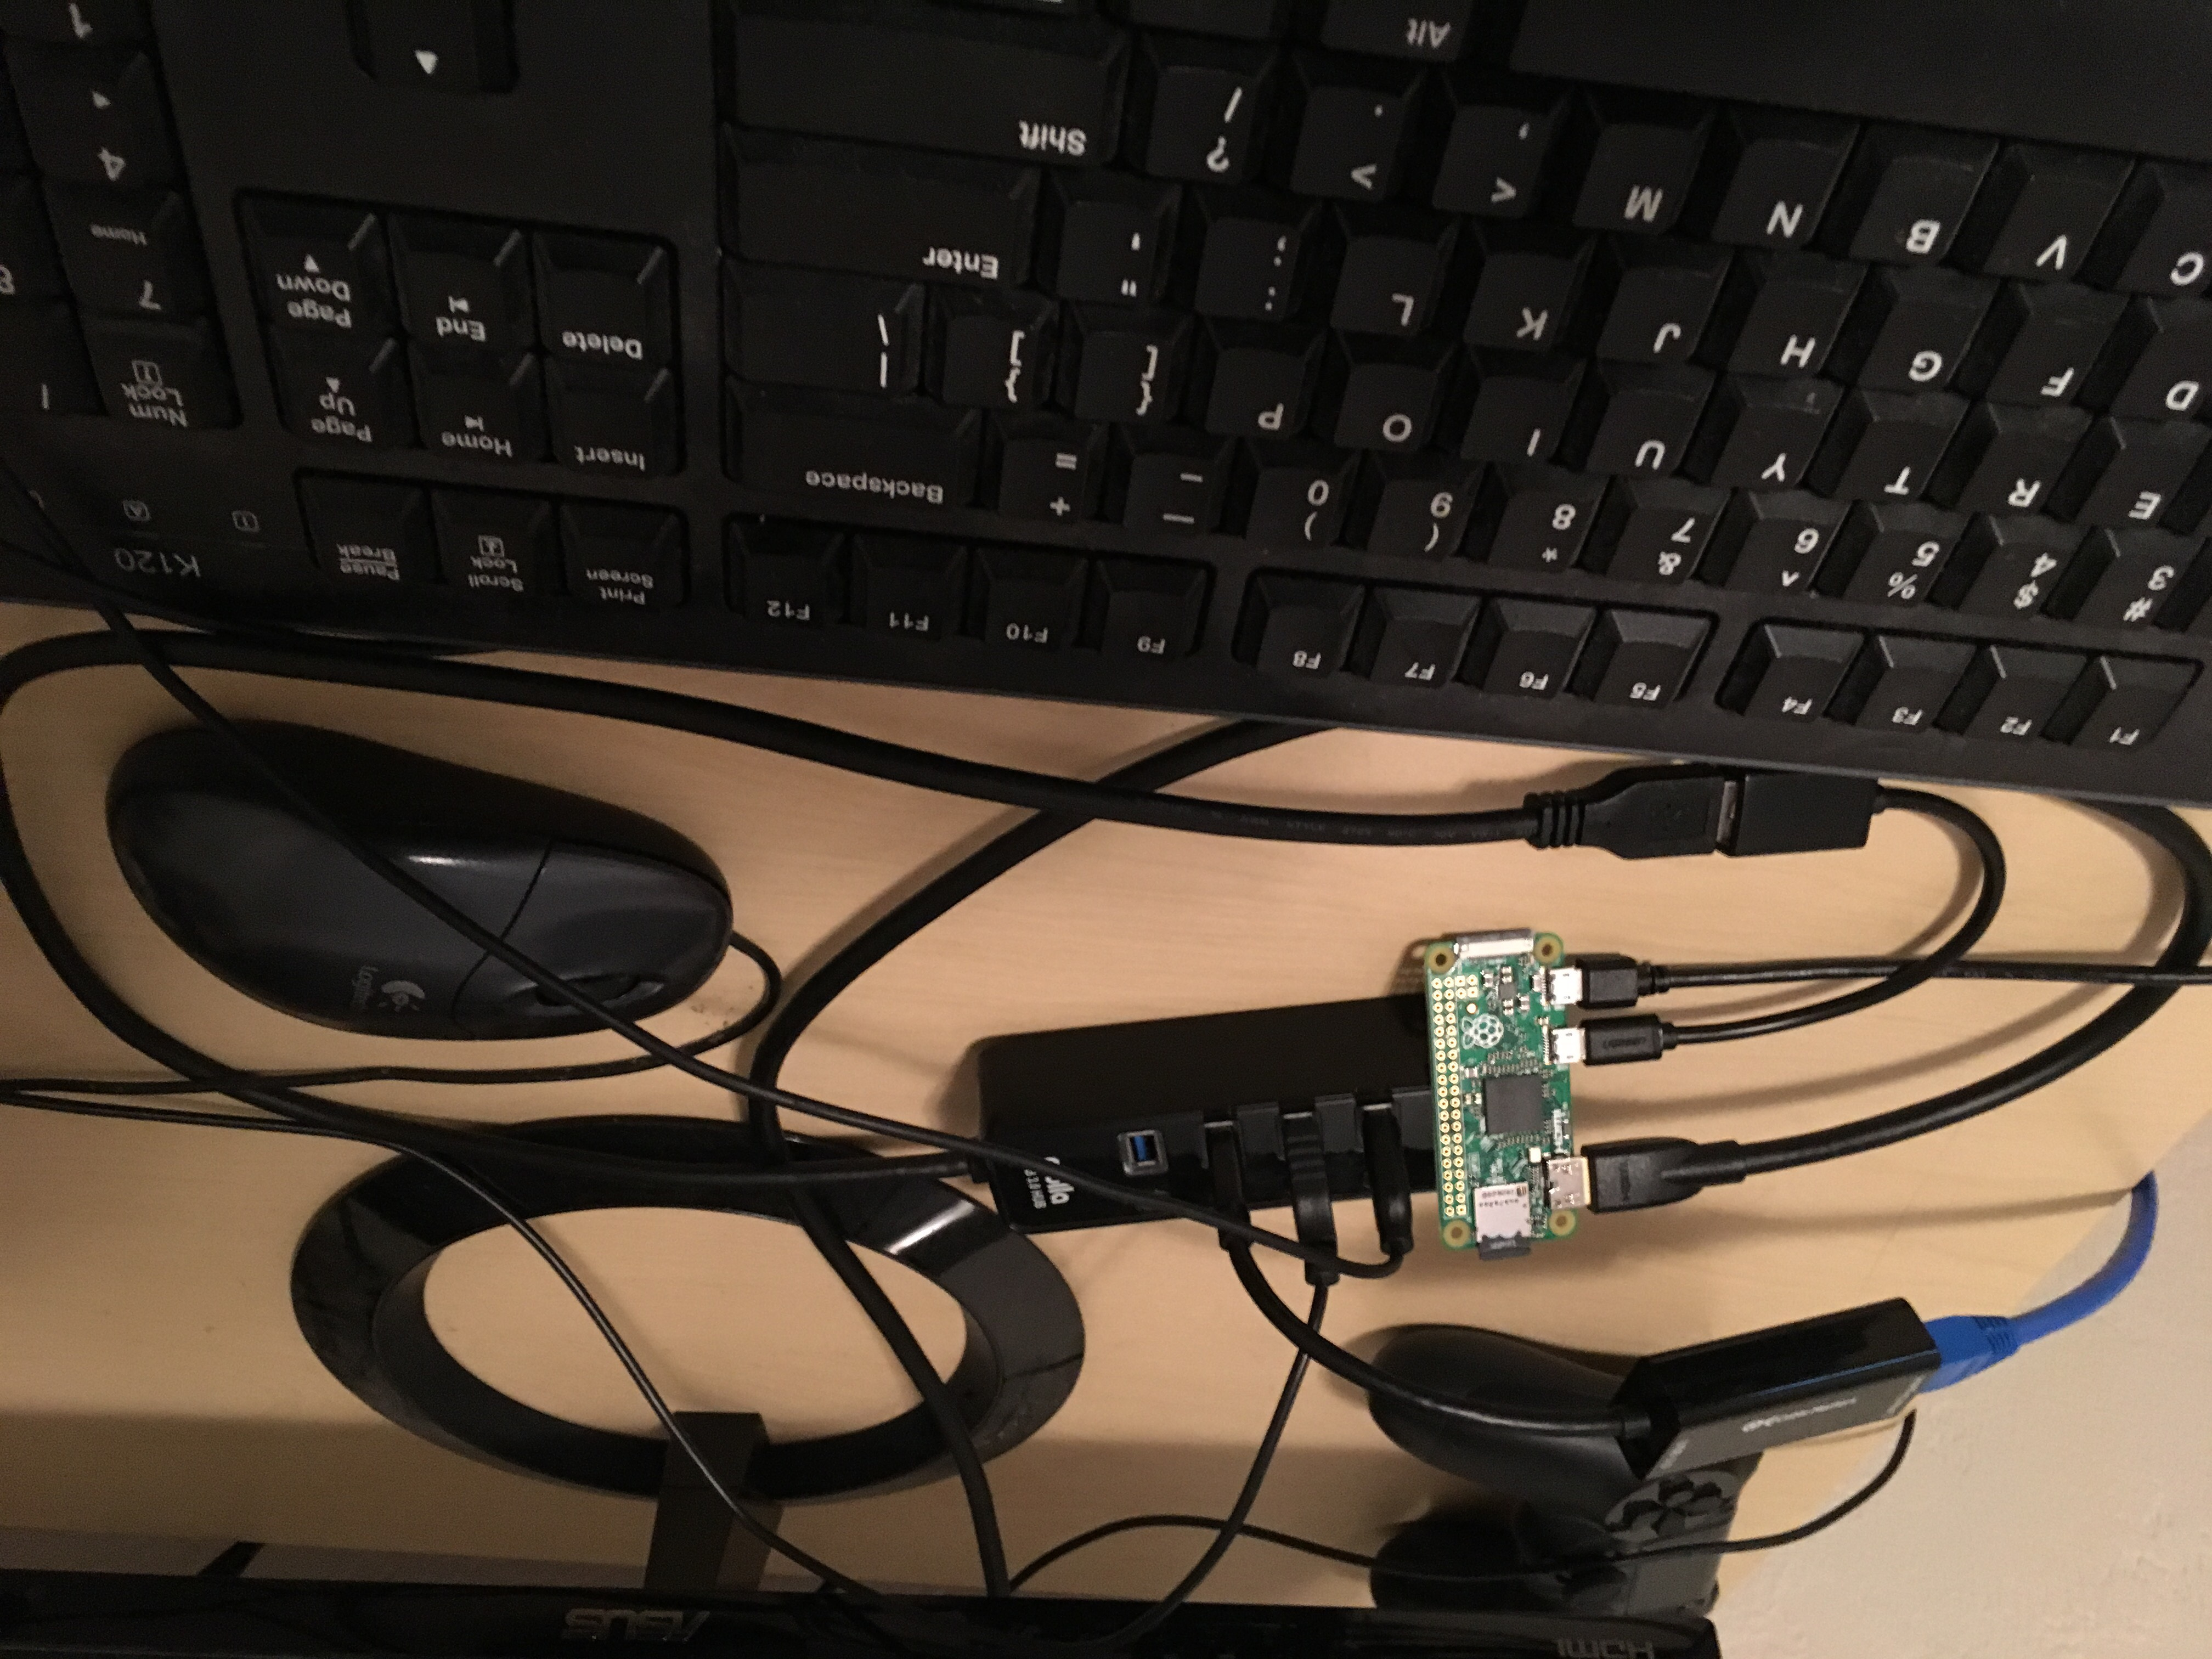
\includegraphics[width=0.45\textwidth,angle=180]{pic1.jpg}
  \caption{All the components needed to use the PI.}
  \label{fig:1}
\end{figure}
\floatstyle{boxed}
\restylefloat{figure}

\par
My most worrying problem is with testing next term. My modules to get unstuck from obstacles and touch the finish pole may perform very poorly in real world tests, and need to be rewritten or improved. This was unavoidable, since tests can only be performed once the rover is completed. Hopefully, the modules perform reasonably well, but it's very important we test the rover as soon as possible next term so we have time to make adjustments. 

\section{Evaluation}
I would call myself the integration expert. I am also in charge of modules within the code, but since the last progress report I have been primarily working on getting our software working on the hardware, so I've worked on merging our software into one piece and primed the hardware to be ready to run our software. Stephen is the obstacle avoidance expert. He is primarily in charge of the obstacle avoidance module, which is one of the more difficult modules to implement. Zach is our visual expert. He is responsible for converting images to binary data to determine where objects are within the image, both for obstacle avoidance and detection. Zach and Stephen are working together closely, because their pieces are closely related. I am also working closely with Zach, because my module to touch the finish pole uses his image detection algorithm to determine where to move the rover. Zhaolong is our navigation expert. He is responsible for our GPS navigation algorithm, which directs the rover towards the finish, and makes periodic course corrections. All members of the team contribute an equal amount. We each work on different pieces, and each piece is essential for the success of the rover at the competition. We also all get along well, and have no issues working together and meeting to discuss the progress of our sections. The only issue I think we have is sometimes we don't have the best communication for immediate questions. We primarily communicate through email, so sometimes we don't immediately respond to each other's questions. Overall, I think we function very well as a development team. 

\section{Reflection of Development Period}
\begin{table}[H]
\begin{tabular}{ |p{0.3\linewidth}|p{0.3\linewidth}|p{0.3\linewidth}|  }
  \hline
  \multicolumn{3}{|c|}{Retrospective} \\
  \hline
  Positives& Deltas &Actions \\
  \hline
  Implemented our software on the actual hardware. &
  Work on better communication methods in the CS group. &
  Get group members to use our slack chat more. \\
  
  No Issues Implementing the software on the hardware. &
  Determine physical tests for the rover to perform. &
  Meet to discuss weak parts of our design to create tests for. \\
  
  The rover is nearly completed. &
  Estabilsh better communication with the ECE Team. &
  Send more updates via email and talk to the ECE Team more. \\

  Met our goals for this term excluding the finished rover. &
  & \\
  \hline
\end{tabular}
\caption{A list of positives, deltas and actions. The deltas and actions are pairs.}
\end{table}
\section{Conclusion}
The final weeks of our project will likely be filled with many revisions to fix assumptions we got wrong before we could test on the hardware. However, we have already completed the vast majority of our project, and all that remains is the final integration onto the hardware, and testing. We will need to determine what tests to put the rover through, in order to determine what parts of our software need to be revised. I look forward to finally seeing our software do what we've been planning for the last two terms. The ME and ECE teams are surely exited to see the completed rover as well. Once we finish testing, all that's left is to wait for the competition, and see how well we do. I'm confident that our rover will perform very well at the competition.

\end{document}
